\documentclass[blue,uncompressed]{beamer}
\usepackage{tikz}
\usepackage{graphicx}
%\usepackage{listingsutf8}
\usepackage{listings}
\usepackage[spanish]{babel}
\usepackage[utf8]{inputenc}
\usepackage{multirow}
\pdfinfo
{
  /Title       (BulletPoint. Tecnología beacon en entornos universitarios.)
  /Creator     (Laura Padrón Jorge)
  /Author      (Laura Padrón Jorge)
  /Subject     (Trabajo de Fin de Grado)
}
%%%%%%%%%%%%%%%%%%%%%%%%%%%%%%%%%%%%%%%%%%%%%%%%%%%%%%%%%%%%%%%%%%%%%%%%%%%%%%%%%%%%%%%%%%%%
% Definiendo colores para los listados de código fuente - Univ. Deusto
\definecolor{violet}{rgb}{0.5,0,0.5}
\definecolor{navy}{rgb}{0,0,0.5}
\definecolor{hellgelb}{rgb}{1,1,0.8}
\definecolor{colKeys}{rgb}{0,0,53}           %%% Todo : check color for keys
\definecolor{colIdentifier}{rgb}{0,0,0}
\definecolor{colComments}{rgb}{1,0,0}
\definecolor{colString}{rgb}{0,0.5,0}
\definecolor{lightlightgray}{rgb}{204,204,204}

\definecolor{marron}       {rgb}{0.496, 0.203, 0.152}
\definecolor{verde-claro}  {rgb}{0.625, 0.734, 0.199}
\definecolor{oscuro}       {rgb}{0.187, 0.141, 0.285}
\definecolor{gris}     	   {rgb}{0.500, 0.500, 0.500}
\definecolor{bgd-listings} {rgb}{0.999, 0.999, 0.900}
\definecolor{gray97}{gray}{.97}
\definecolor{gray75}{gray}{.75}
\definecolor{gray45}{gray}{.45}
\definecolor{gray}{gray}{.45}
%%%%%%%%%%%%%%%%%%%%%%%%%%%%%%%%%%%%%%%%%%%%%%%%%%%%%%%%%%%%%%%%%%%%%%%%%%%%%%%%%%%%%%%%%%%%
\lstloadlanguages{Java}
\lstloadlanguages{XML}
\lstset{
	float=hbp,
		language = Java,
			morekeywords={hicuda,global,alloc,shape,kernel,thread,loop_partition,tblock,over_tblock,over_thread,kernel_end,copyout,free,data,region,task,input,inout,output,pragma,omp,parallel,reduction,private,shared,target,device,copy_in,copy_out,acc,kernels,loop,copyin,copy,pcopy,pcopyin,collapse,gang,worker,independent,firstprivate,endfor,in},
				%\emph      ={omp,parallel,reduction,private,shared},
				xleftmargin=5.0ex,    % Margen izq. para que los números de línea se vean
				emphstyle=\textbf,
        basicstyle=\ttfamily\scriptsize,
        identifierstyle=\color{colIdentifier},
        keywordstyle=\color{colKeys},
        stringstyle=\color{colString},
        commentstyle=\color[rgb]{0.133,0.545,0.133},
        columns=flexible,
        tabsize=4,
        frame=single,
        extendedchars=true,
        showspaces=false,
        showstringspaces=false,
        numbers=left,
        numberstyle=\tiny,
        breaklines=true,
        backgroundcolor=\color{lightlightgray},
        breakautoindent=true,
        captionpos=b
        morecomment=[l][\color{colKeys}]{\#}
}
%%%%%%%%%%%%%%%%%%%%%%%%%%%%%%%%%%%%%%%%%%%%%%%%%%%%%%%%%%%%%%%%%%%%%%%%%%%%%%%%%%%%%%%%%%%%
\mode<handout>
{
	\usepackage{pgfpages}
	\pgfpagesuselayout{2 on 1}[a4paper,border shrink=5mm]
	\setbeamercolor{background canvas}{bg=black!0}
	\setbeameroption{show notes}
}

\mode<presentation>
{
	\usetheme{Madrid}
	\usecolortheme{ull}
	\setbeamercovered{transparent}
	%\logo{  % Logo ULL en esquina inferior derecha
	%    \includegraphics[width=.25\textwidth]{FIGURES/logoull-oficial.png}
	%}
}
%%%%%%%%%%%%%%%%%%%%%%%%%%%%%%%%%%%%%%%%%%%%%%%%%%%%%%%%%%%%%%%%%%%%%%%%%%%%%%%%%%%%%%%%%%%%
\AtBeginSection[]
{
	\begin{frame}<beamer>
		\frametitle{Outline}
		\tableofcontents[currentsection,currentsubsection]
	\end{frame}
}
%%%%%%%%%%%%%%%%%%%%%%%%%%%%%%%%%%%%%%%%%%%%%%%%%%%%%%%%%%%%%%%%%%%%%%%%%%%%%%%%%%%%%%%%%%%%
\title{\textbf{BulletPoint}}
\subtitle{Tecnología beacon en entornos universitarios}
\author[Laura Padrón Jorge]
{
	\textbf{Laura Padrón Jorge}
	%\alert{Francisco~de Sande} \\
	%\url{fsande@ull.es}
}
\institute[ULL]

\date[Trabajo de Fin de Grado]{\textsc{Trabajo de Fin de Grado}     \\
                           La Laguna, 15 de Julio, 2016}
\subject{TFG}

\AtBeginSection[]
{
	\frame<handout:0>
		{
			\frametitle{Índice}
			\tableofcontents[current]
		}
}
%%%%%%%%%%%%%%%%%%%%%%%%%%%%%%%%%%%%%%%%%%%%%%%%%%%%%%%%%%%%%%%%%%%%%%%%%%%%%%%%%%%%%%%%%%%%
\newcommand{\BulletPoint}{\texttt{BulletPoint{}}}

\setbeamerfont{title}{size=\Large,shape=\sffamily}
\setbeamerfont{author}{size=\small,shape=\sffamily}
\setbeamerfont{institute}{size=\scriptsize,shape=\sffamily}
\setbeamerfont{date}{size=\scriptsize,shape=\sffamily}
%%%%%%%%%%%%%%%%%%%%%%%% Title Page %%%%%%%%%%%%%%%%%%%%%%%%%%%%%%%%%%%%%%%%%%%%%%%%%%%%%%%%%%%%%%%%%%%%
\defbeamertemplate*{title page}{AGH}[1][]
{
  \vbox{}
  %\vspace*{2.3cm}
  \vfill 
\includegraphics[width=0.15\linewidth]{Images/logos/logo_vertical}
    \vfill
  %\hspace*{1.8cm}
  \begin{columns}
    \begin{column}{0.6\textwidth}
      \begin{beamercolorbox}[sep=8pt,#1]{title}
	\centering{\usebeamerfont{title}\inserttitle\par}
	\ifx\insertsubtitle\@empty%
	\else%
	  \vskip0.25em%
	  {\usebeamerfont{subtitle}\usebeamercolor[fg]{subtitle}\insertsubtitle\par}%
	\fi%
	
      \end{beamercolorbox}%
      \vskip1em\par
      \hspace*{2.35cm}
      \begin{beamercolorbox}[sep=8pt,#1]{author}
	\usebeamerfont{author}\insertauthor
      \end{beamercolorbox}
      \vskip1em\par
      \hspace*{2.35cm}
      \begin{beamercolorbox}[sep=8pt,#1]{institute}
	\usebeamerfont{institute}\insertinstitute
      \end{beamercolorbox}
      \hspace*{2.35cm}
      \begin{beamercolorbox}[sep=8pt,#1]{date}
	\usebeamerfont{date}\insertdate
      \end{beamercolorbox}\vskip0.5em
    \end{column}
    
    \begin{column}{0.4\textwidth}
      \hfill 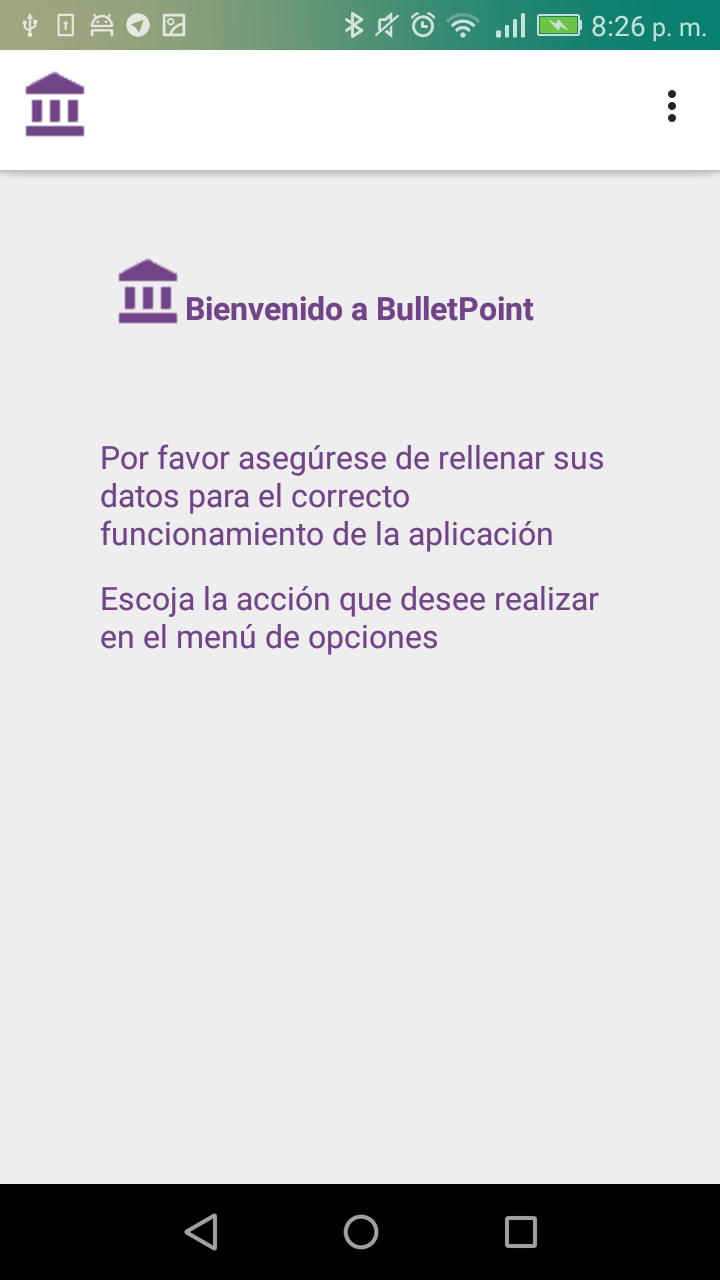
\includegraphics[width=0.8\linewidth]{Images/App/menuPrincipal.png}
    \end{column}
  \end{columns}
    %\hfill 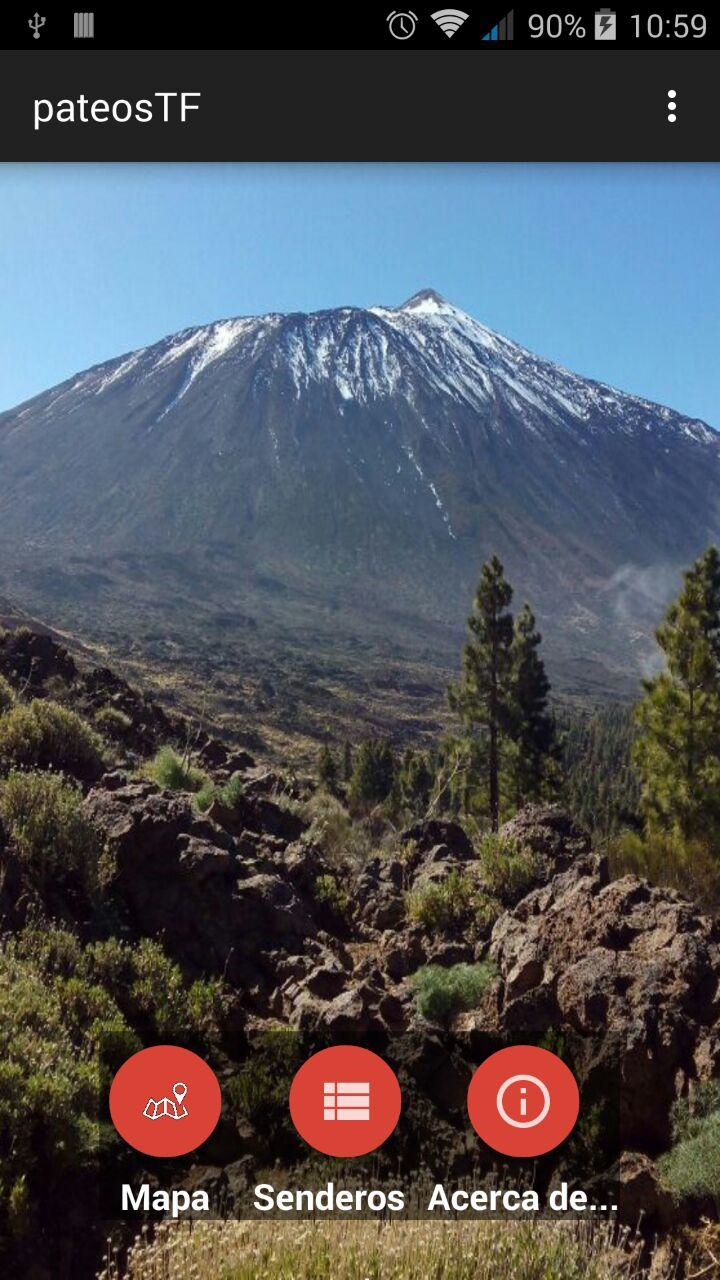
\includegraphics[width=0.2\linewidth]{Images/varios/MainActivity.png}
    %{\usebeamercolor[fg]{titlegraphic}\inserttitlegraphic\par}
	%	\vfill \includegraphics[width=0.3\linewidth]{FIGURES/logos/nwo}
	%	\hfill \includegraphics[width=0.17\linewidth]{FIGURES/logos/stw}
	%	\hfill \includegraphics[width=0.2\linewidth]{FIGURES/logos/ipn.jpg}
  %\vfill
}
%%%%%%%%%%%%%%%%%%%%%%%%%%%%%%%%%%%%%%%%%%%%%%%%%%%%%%%%%%%%%%%%%%%%%%%%%%%%%%%%%%%%%%%%%%%%
% Slide numbers. 
%\expandafter\def\expandafter\insertshorttitle\expandafter{%
%  \insertshorttitle\hfill%
%  \insertframenumber\,/\,\inserttotalframenumber
%}
%%%%%%%%%%%%%%%%%%%%%%%%%%%%%%%%%%%%%%%%%%%%%%%%%%%%%%%%%%%%%%%%%%%%%%%%%%%%%%%%%%%%%%%%%%%%
\begin{document}
	%\frame{\titlepage}
	\begin{frame}[plain]
	\titlepage
	\end{frame}

	\frame{\frametitle{Índice}\tableofcontents}
		\section{Introducción}
			\begin{frame}
    \frametitle{Introducción}
    %\block{Objetivo del TFG}
    \begin{itemize}
	\item \textbf{Tutor Trabajo Fin de Grado:} Francisco de Sande González
        \item \textbf{Línea de trabajo del proyecto:} Programación de aplicaciones interactivas en {\it Android}.
    \end{itemize}
    %\endblock{}
        {\usebeamercolor[fg]{titlegraphic}\inserttitlegraphic\par}
		\vfill 
\includegraphics[width=0.2\linewidth]{Images/logos/aruba_networks}
		\hfill %
		
\includegraphics[width=0.2\linewidth]{Images/logos/android_logo}
		\hfill 
\includegraphics[width=0.35\linewidth]{Images/logos/couchbase_logo}
\end{frame}
% -------------------------------------------------------------------------
\begin{frame}
	\frametitle{Introducción}
	\block{Objetivos}
		\begin{itemize}
			\item Desarrollo de un proyecto de Ingeniería.
			\item Programación de aplicaciones en Android.
			\item Investigación de la tecnología beacon.
			\item Repositorio online.
			\item Creación de una memoria técnica.
			\item \textit{LaTeX}.
		\end{itemize}
	\endblock{}
\end{frame}
% -------------------------------------------------------------------------
		\section{Herramientas y Tecnologías utilizadas}
			\begin{frame}
	\frametitle{Herramientas y Tecnologías utilizadas}
	\block{ Android Studio}
		\begin{itemize}
			\item Entorno de desarrollo integrado.
			\item Gradle.
			\item Sistema de depuración sencillo e intuitivo.
		\end{itemize}
		Descarga en: \texttt{https://developer.android.com/studio/index.html}
	\endblock{}
\end{frame}

%------------------------------------------------------------------
\begin{frame}
	\frametitle{Herramientas y Tecnologías utilizadas}
	\block{\it Beacons}
		\begin{itemize}
			\item {\it ¿Qué es un beacon?}.
			\item {\it ¿Cómo funcionan estos dispositivos?}.
			\item {\it ¿Qué rango de alcance poseen?}.
			\item {\it ¿Con qué dispositivos móviles son compatibles?}.
			\item {\it ¿Qué ventajas y desventajas presenta su uso?}.
			\item {\it ¿Qué usos se ha dado a esta tecnología?}.
		\end{itemize}
	\endblock{}
\end{frame}

%------------------------------------------------------------------

\begin{frame}
	\frametitle{Herramientas y Tecnologías utilizadas}
	\begin{columns}
		\begin{column}{0.6\textwidth}
			\block{\it ¿Qué es un beacon?}
			\begin{itemize}
				\item Pequeño dispositivo que emite señales utilizando Bluetooth.
				\item Señales unidireccionales que emiten información.
				\item Recibidas por dispositivos móviles.
				\item Aplicaciones programadas para recibir estas señales.
			\end{itemize}
			\endblock{}
		\end{column}
		\begin{column}{0.4\textwidth}
			\vfill 
			\begin{center}
				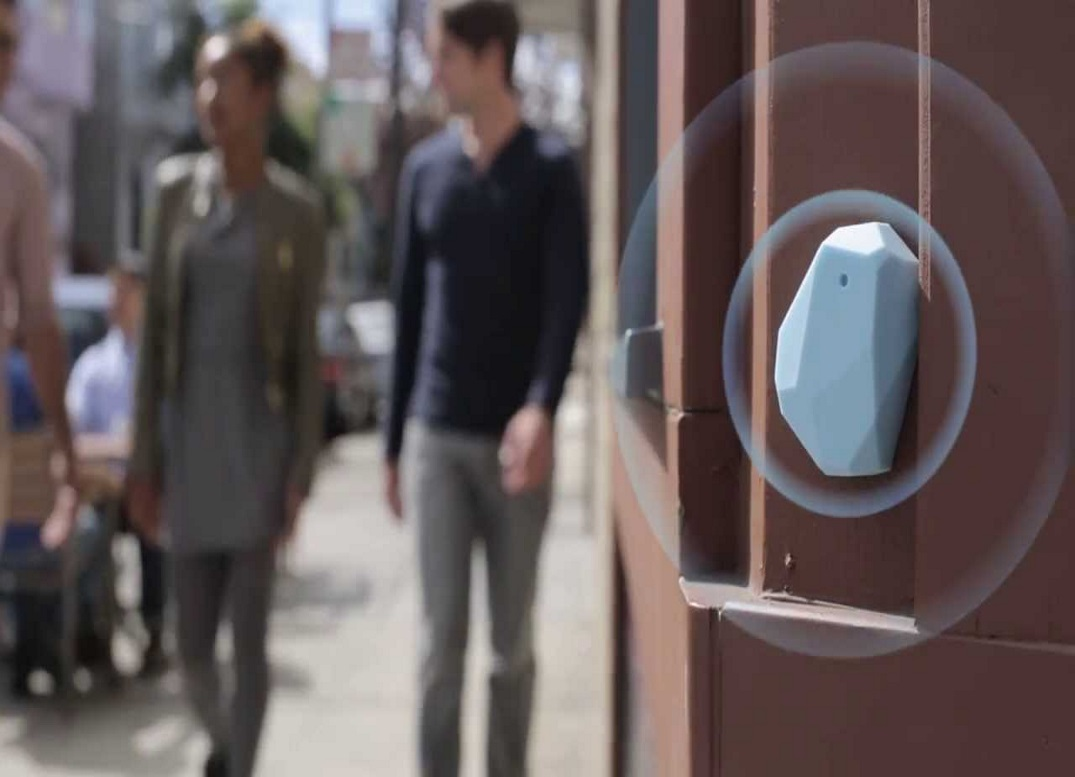
\includegraphics[width=0.8\linewidth]{Images/estimoteBeacon}
			\end{center}
		\end{column}
	\end{columns}
\end{frame}

%------------------------------------------------------------------
\begin{frame}
	\frametitle{Herramientas y Tecnologías utilizadas}
		\begin{columns}
			\begin{column}{0.6\textwidth}
				\block{\it ¿ Como funcionan estos dispositivos?}
					\begin{itemize}
						\item {Los beacons usan Bluetooth Low Energy (BLE).}
						\item {Los beacons funcionan con baterías.}
						\item {Transmiten identificadores cortos.}
					\end{itemize}
				\endblock{}
			\end{column}
			\begin{column}{0.4\textwidth}
				\vfill 
					\begin{center}
						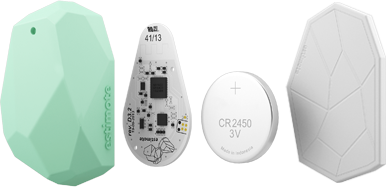
\includegraphics[width=0.8\linewidth]{Images/estimoteBeaconInside}
					\end{center}
			\end{column}
		\end{columns}
\end{frame}		
		


\begin{frame}
	\frametitle{Herramientas y Tecnologías utilizadas}
	\begin{columns}
			\begin{column}{0.6\textwidth}
				\block{\it ¿Qué rango de alcance poseen?}
					\begin{itemize}
						\item {Rango de 70 metros de radio sin obstáculos.}
						\item {Este rango puede disminuir signicativamente.}
						\item {Las aplicaciones suelen definir acciones en tres rangos.}
						\item {Es posible lanzar acciones a una distancia determinada.}
					\end{itemize}
				\endblock{}
			\end{column}
			\begin{column}{0.4\textwidth}
				\vfill 
					\begin{center}
						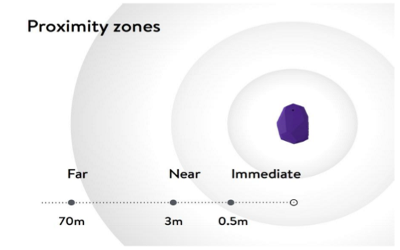
\includegraphics[width=0.8\linewidth]{Images/beaconsRange}
					\end{center}
			\end{column}
	\end{columns}
\end{frame}

%------------------------------------------------------------------

\begin{frame}
	\frametitle{Herramientas y Tecnologías utilizadas}
	\begin{columns}
			\begin{column}{0.6\textwidth}
				\block{\it ¿ Con qué dispositivos móviles son compatibles?}
					\begin{itemize}
						\item {Todos los dispositivos que soporten BLE.}
						\item {En IOS7 o superior.}
						\item {En dispositivos Android.}
					\end{itemize}
				\endblock{}
			\end{column}
			\begin{column}{0.4\textwidth}
				\vfill 
					\begin{center}
						
\includegraphics[width=0.8\linewidth]{Images/arubaBeacons}
					\end{center}
			\end{column}
	\end{columns}
\end{frame}

%--------------------------------------------------------------------

\begin{frame}
	\frametitle{Herramientas y Tecnologías utilizadas}
	\block{\it ¿Que ventajas y desventajas tienen con respecto a otras tecnologías?}
		\begin{columns}
			\begin{column}{0.9\textwidth}
				\block{\it Ventajas}
					\begin{itemize}
						\item {BLE menos batería que GPS.}
						\item {Funciona en el interior de los edificios.}
						\item {En dispositivos Android.}
					\end{itemize}
				\endblock{}			
				\block{\it Desventajas}
					\begin{itemize}
						\item {Dependen de aplicaciones instaladas.}
						\item {Es necesario activar el Bluetooth.}
						\item {Su utilidad depende de la voluntad de terceros.}
					\end{itemize}
				\endblock{}
			\end{column}
		\end{columns}
	\endblock{}
\end{frame}


\begin{frame}
	\frametitle{Herramientas y Tecnologías utilizadas}
	\block{\it ¿Qué usos se le ha dado a esta tecnología hasta ahora?}
		\begin{columns}
			\begin{column}{0.3\textwidth}
				Clevedon School App
				\vspace{3mm}
				\vfill 
					\begin{center}
						
\includegraphics[width=0.8\linewidth]{Images/ClevedonApp}
					\end{center}
			\end{column}
			\begin{column}{0.3\textwidth}
				Levi's Stadium App
				\vspace{3mm}
				\vfill 
					\begin{center}
						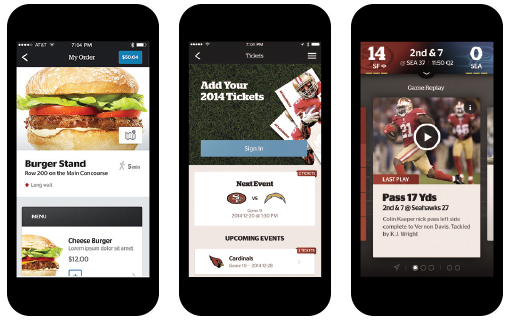
\includegraphics[width=0.8\linewidth]{Images/LevisStadium}
					\end{center}
			\end{column}
			\begin{column}{0.3\textwidth}
				OrlandoInt'l Airport
				\vspace{3mm}
				\vfill 
					\begin{center}
						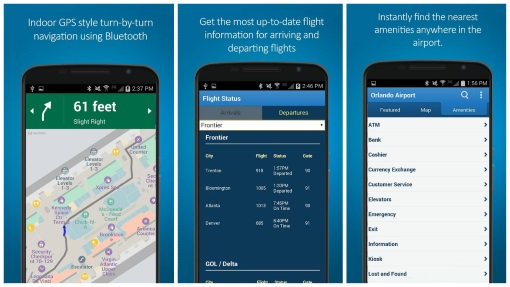
\includegraphics[width=0.8\linewidth]{Images/orlandoAirport}
					\end{center}
			\end{column}
		\end{columns}
	\endblock{}
\end{frame}

\begin{frame}
	\frametitle{Herramientas y Tecnologías utilizadas}
		\block{\it CouchBase Server}
			\begin{itemize}
				\item {¿Qué es?}
				\item {¿Qué nos ha permitido?}
				\item {¿Por qué se ha decidido utilizar esta tecnología?}
			\end{itemize}
		\endblock{}
		\vfill 
			\begin{center}
				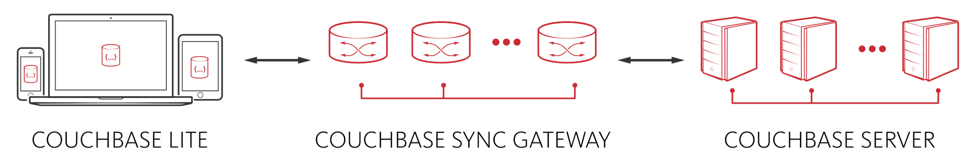
\includegraphics[width=0.8\linewidth]{Images/couchBase}
			\end{center}
\end{frame}

\begin{frame}
	\frametitle{Herramientas y Tecnologías utilizadas}
		\block{\it La librería AltBeacon}
			Se puede definir AltBeacon como una especificación que:
			\begin{itemize}
				\item {Define el formato del protocolo publicitario a través de BLE.}
				\item {Intenta crear un mercado abierto y competitivo para implementaciones usando proximidad.}
				\item {Puede ser utilizada gratuitamente, sin cuotas ni compromisos.}
				\item {No favorece a ningún proveedor sobre otro.}
			\end{itemize}
		\endblock{}
		\block{\it Funcionamiento}
			\begin{columns}
				\begin{column}{0.7\textwidth}
					\begin{itemize}
						\item {Monitorizacion(\textit{``Monitoring''})}
						\item {Rastreo (\textit{``Ranging''})}
					\end{itemize}
				\end{column}
				\begin{column}{0.3\textwidth}
					\vfill 
					\begin{center}
						
\includegraphics[width=0.5\linewidth]{Images/logos/altBeacon}
					\end{center}
				\end{column}
			\end{columns}
		\endblock{}
\end{frame}

\begin{frame}
	\frametitle{Herramientas y Tecnologías utilizadas}
	\begin{columns}
			\begin{column}{0.6\textwidth}
				\block{\it El algoritmo de trilateración}
					\begin{itemize}
						\item {Es un método matemático para determinar las posiciones relativasde objetos.}
						\item {Utiliza las localizaciones de dos o más puntos y las distancias entre el sujeto y cada punto.}
						\item {En un plano bidimensional, se necesitan al menos 3 puntos de referencia.}
					\end{itemize}
				\endblock{}
			\end{column}
			\begin{column}{0.4\textwidth}
				\vfill 
					\begin{center}
						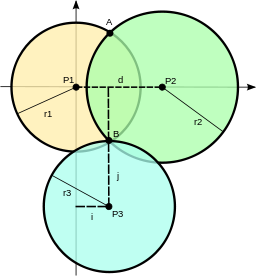
\includegraphics[width=0.8\linewidth]{Images/trilateration}
					\end{center}
			\end{column}
	\end{columns}
\end{frame}

\begin{frame}
	\frametitle{Algoritmo de trilateración utilizado}
	\lstinputlisting{Code/trilaterate.java}
\end{frame}

%--------------------------------------------------------------------

		\section{Beacons en entornos universitarios}
			\begin{frame}
	\frametitle{Beacons en entornos universitarios}
			\block{\it Introducción}
				\begin{itemize}
					\item Posibilidades amplias para apps en entornos universitarios.
					\item Cada universidad intenta tener su propia aplicación siguiendo un patrón similar.
					\item Estas aplicaciones se centran en ofrecer servicios propios.
				\end{itemize}
			\endblock{}
\end{frame}

%------------------------------------------------------------------

\begin{frame}
	\frametitle{Beacons en entornos universitarios}
		\begin{columns}
			\begin{column}{0.6\textwidth}
				\block{\it Posibles casos de uso en entornos universitarios}
					\begin{itemize}
						\item Guía a través del campus de la universidad.
						\item Acceso al parking y recuento de número de plazas disponibles.
						\item Gestión de eventose información, entrada automática.
						\item Actividades interactivas por el campus, jornadas de acogida u otros eventos.
						\item Despacho del profesorado e información
					\end{itemize}
				\endblock{}
			\end{column}
			\begin{column}{0.4\textwidth}
				\vfill 
				\begin{center}
					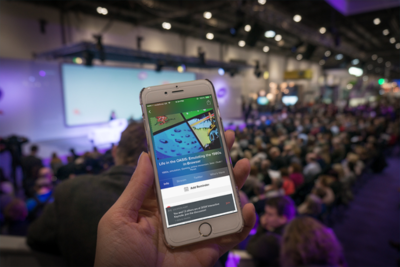
\includegraphics[width=0.9\linewidth]{Images/BeaconEvent}
				\end{center}
			\end{column}		
		\end{columns}
\end{frame}


%---------------------------------------------------------------------

\begin{frame}
	\frametitle{Beacons en entornos universitarios}
		\begin{columns}
			\begin{column}{0.6\textwidth}
				\block{\it Posibles casos de uso en entornos universitarios}
					\begin{itemize}
						\item Control de asistencia.
						\item Localizaciónde transporte público, horarios e informaciónde la parada.
						\item Biblioteca informativa.
						\item Control de acceso a instalaciones.
						\item Información y descuentos para usuarios de la app.
						\item Descarga automática de material.
					\end{itemize}
				\endblock{}
			\end{column}
			\begin{column}{0.4\textwidth}
				\vfill 
				\begin{center}
					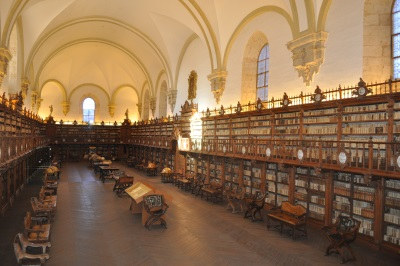
\includegraphics[width=0.9\linewidth]{Images/BibliotecaSalamanca}
				\end{center}
			\end{column}		
		\end{columns}
\end{frame}

		\section{La aplicación \BulletPoint}
			\begin{frame}
	\frametitle{La aplicación \BulletPoint{}}
	\begin{columns}
		\begin{column}{0.6\textwidth}
			\block{Localización de transporte público, horarios e información de la parada}
			\begin{itemize}
				\item Objetivo.
				\item Despliegue.
				\item Funcionamiento.
				\item Dificultades.
				\item Ampliación.
			\end{itemize}
			\endblock{}
		\end{column}
		\begin{column}{0.4\textwidth}
			\vfill 
			\begin{center}
				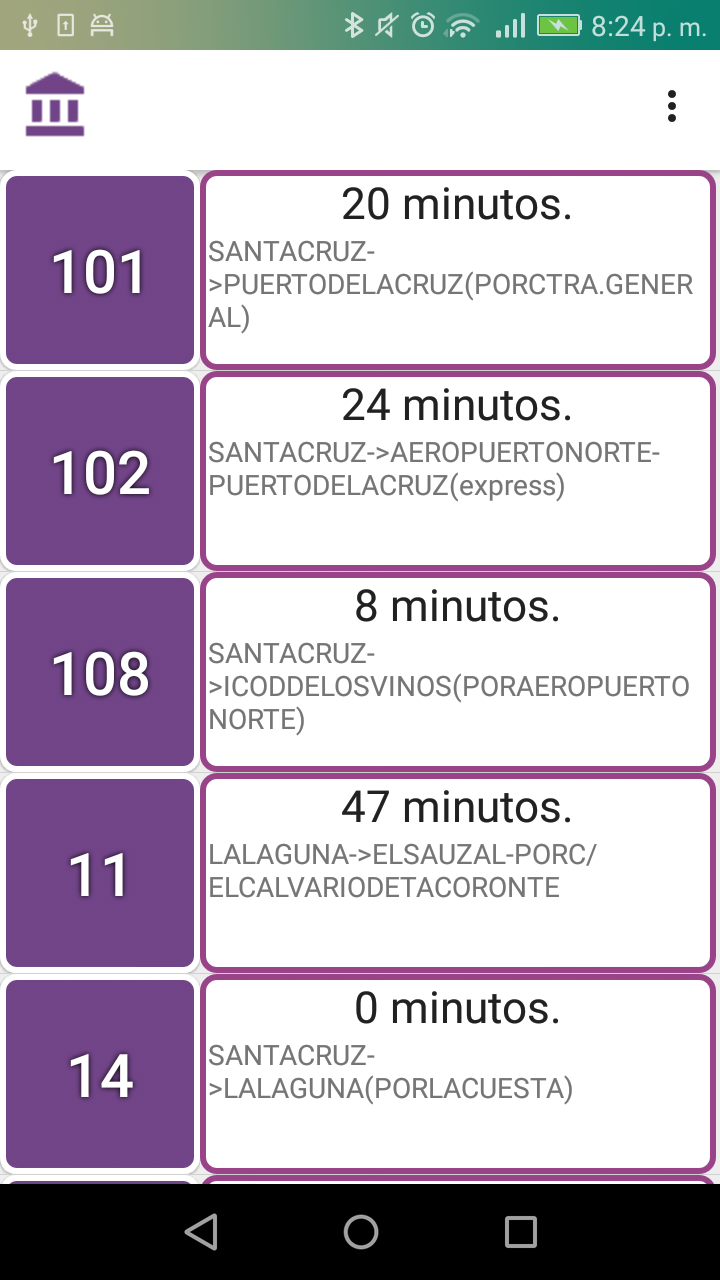
\includegraphics[width=0.8\linewidth]{Images/App/Autobuses}
			\end{center}
		\end{column}
	\end{columns}
\end{frame}

%--------------------------------------------------------------------

\begin{frame}
	\frametitle{Asociación de MAC a identificador de parada}
	\lstinputlisting{Code/BeaconBusStop.java}
\end{frame}

%--------------------------------------------------------------------

\begin{frame}
	\frametitle{Petición API TITSA}
	\lstinputlisting{Code/HttpClientTitsaJsoup.java}
\end{frame}

%--------------------------------------------------------------------

\begin{frame}
	\frametitle{La aplicación \BulletPoint{}}
	\begin{columns}
		\begin{column}{0.6\textwidth}
			\block{Gestión de eventos e información}
			\begin{itemize}
				\item Objetivo.
				\item Despliegue.
				\item Funcionamiento.
				\item Dificultades.
				\item Ampliación.
			\end{itemize}
			\endblock{}
		\end{column}
		\begin{column}{0.4\textwidth}
			\vfill 
			\begin{center}
				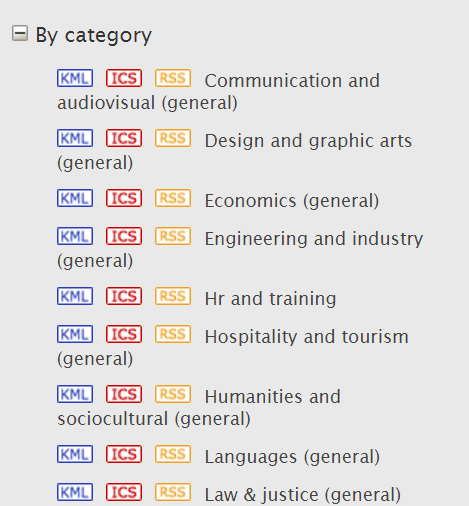
\includegraphics[width=0.7\linewidth]{Images/eventsRss}
			\end{center}
		\end{column}
	\end{columns}
\end{frame}

%--------------------------------------------------------------------

\begin{frame}
	\frametitle{Asociación de MAC a enlace RSS}
	\lstinputlisting{Code/RssBeaconInfo.java}
\end{frame}

%--------------------------------------------------------------------

\begin{frame}
	\frametitle{La aplicación \BulletPoint{}}
		\block{Control de asistencia}
		\begin{itemize}
			\item Objetivo.
			\item Despliegue.
			\item Funcionamiento.
			\item Dificultades.
			\item Ampliación.
		\end{itemize}
		\endblock{}
\end{frame}

%--------------------------------------------------------------------

\begin{frame}
	\frametitle{Preferencias de usuario}
	\lstinputlisting{Code/preferences.xml}
\end{frame}

%--------------------------------------------------------------------

\begin{frame}
	\frametitle{Comprobando la localización en el área}
	\lstinputlisting{Code/scanAtt.java}
\end{frame}

%--------------------------------------------------------------------

\begin{frame}
	\frametitle{La aplicación \BulletPoint{}}
		\block{Guía a través del campus de la universidad}
		\begin{itemize}
			\item Objetivo.
			\item Despliegue.
			\item Funcionamiento.
			\item Dificultades.
			\item Ampliación.
		\end{itemize}
		\endblock{}
\end{frame}

%--------------------------------------------------------------------

\begin{frame}
	\frametitle{Mostrar la posición del usuario en la imagen}
	\lstinputlisting{Code/threeMainFunctionTrilaterate.java}
\end{frame}

\begin{frame}
	\frametitle{La aplicación \BulletPoint{}}
	\begin{columns}
		\begin{column}{0.6\textwidth}
			\block{Acceso al parking}
			\begin{itemize}
				\item Objetivo.
				\item Despliegue.
				\item Funcionamiento.
				\item Dificultades.
				\item Ampliación.
			\end{itemize}
			\endblock{}
		\end{column}
		\begin{column}{0.4\textwidth}
			\vfill 
			\begin{center}
				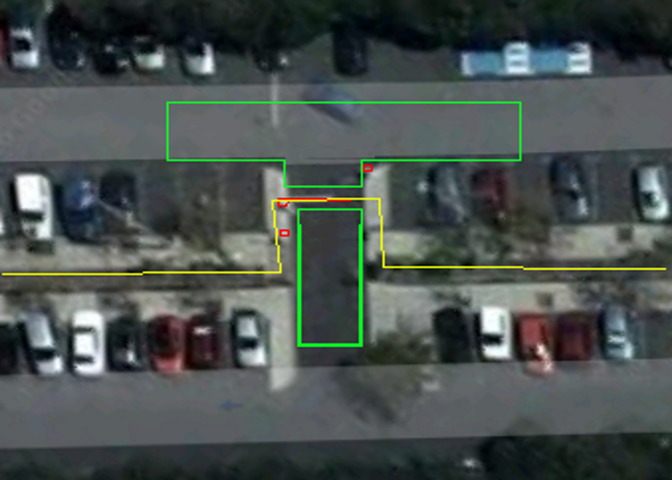
\includegraphics[width=0.9\linewidth]{Images/parking}
			\end{center}
		\end{column}
	\end{columns}
\end{frame}

%--------------------------------------------------------------------

\begin{frame}
	\frametitle{La aplicación \BulletPoint{}}
		Vídeo demostrativo de la aplicación \BulletPoint{}
\end{frame}
		\section{Despliegue}
			\begin{frame}
  \frametitle{Despliegue}
  \block{Repositorio de la aplicación}
    \begin{itemize}
		\item La aplicación ha sido almacenada en el repositorio GitHub como parte del PATFL.
    \item Se encuentra en GitHub: https://github.com/ccetsii/BulletPoint 
    \end{itemize}
  \endblock{}
\end{frame}
		\section{Presupuesto}	
			\begin{frame}
	\frametitle{Presupuesto}
	\block{Coste de los dispositivos}
		\begin{itemize}
			\item Autobuses: inversión de 500 euros y cubriríamos 20 paradas de autobús.
			\item Eventos: Para las 10 zonas de eventos se invertirían 250 euros.
			\item Aparcamientos: 8 aparcamientos. Mínimo 3 beacons por recinto. Desembolso de 600 euros.
			\item Asistencia y guía: cubriendo todos los edificios de la ULL se necesitarían unos 100 beacons, el importe asciende a 2500 euros.
			\item Total: 154 dispositivos con un coste de 3.850 euros.
		\end{itemize}
	\endblock{}
\end{frame}


\begin{frame}
	\frametitle{Presupuesto}
	\block{Despliegue de los dispositivos}
		\begin{itemize}
			\item Tarifa: 12,40 euros por hora trabajada.
			\item Se necesitaran 2 especialistas trabajando durante un mes a jornada completa (8 horas). 
			\item Total: 3.968 euros.
		\end{itemize}
	\endblock{}
\end{frame}


\begin{frame}
	\frametitle{Presupuesto}
	\block{Servidor para el almacenamiento de información}
		\begin{enumerate}
			\item Compra del servidor dedicado junto con el soporte y configuración servidor (cuota anual) : 1300 + 250 = 1.550 euros.
			\item Configuración de un servidor ya disponible en la Universidad (sin cuota anual de soporte ni mantenimiento): 550 euros.
		\end{enumerate}
	\endblock{}
\end{frame}


\begin{frame}
	\frametitle{Presupuesto}
	\block{Mantenimiento de la aplicación}
		\begin{itemize}
			\item Ofrecemos un especialista programador en Android.
			\item Este mantenimiento no incluye nuevas funcionalidades.
			\item Tarifa: 21.600 euros anuales netos durante el primer año y a 18.000 euros en adelante.
		\end{itemize}
	\endblock{}
\end{frame}
		\section{Summary and conclusions}
			\begin{frame} [fragile]
	\frametitle{Summary and conclusions}
	\block{Conclusions}
		Nowadays, beacon technology is still on a development phase.By itself can be quite limited due to its functioning.The physical and positional limitations require a deep analysis in order to place devices the best way.
		
		\bigskip
		On the other hand, each specific beacon provider tries to use his own SDKs to develop the applications.
		
		\bigskip
		The solution to this problem, in this case, has been found on the AltBeaconlibrary, which tries to bring close to developers this technology.
		
		\bigskip
	The achievement of this Final Year Project is to show that, many apps able to work with this technology exist or can be developed.
	
		\bigskip
		For now, we will keep on testing this technology and watching it grow.

	\endblock{}
\end{frame}
		\begin{frame}
  \frametitle{Agradecimientos}
  \block{Agradecimientos}
    \begin{itemize}
    \item Servicios TIC, en especial a Don Juan Carlos Hernández Perdomo.
		\item Don Alberto Morales de la empresa Galotecnia Redes Sistemas y Servicios S.L.
		\item Transportes Interurbanos de Tenerife S.A. (TITSA).
    \end{itemize}
  \endblock{}
\end{frame}
		\include{Capitulos/Cap9_final}
%%%%%%%%%%%%%%%%%%%%%%%%%%%%%%%%%%%%%%%%%%%%%%%%%%%%%%%%%%%%%%%%%%%%%%%%%%%%%%%%%%%%%%%%%%%%
\end{document}